%%% Fiktivní kapitola s ukázkami sazby

\chapter{Problémová oblast}{\tiny }

Sledování a popis životního cyklu ptáků, vědecká disciplína nazývaná ornitologie, je poměrně starou vědeckou disciplínou s kořeny již ve starověku. Jedním z prvních dochovaných textů zabývajícím se popisu života ptáků je Aristotelova \emph{Historia Animalium} v roce 350 př. n. l \cite{historiaAnimalium}, která podrobně popisovala mimojiné i ptačí migrace. Ornitologie se postupně rozvíjela -- zaváděly se taxonomie ptactva, studovala se ptačí anatomie, ale spousta otázek spojena s chováním ptáků zůstavala nezodpovězena. V roce 1805 se Americký ornitolog John James Audubon údajně snažil prokázat, že se každým rokem na jeho farmu vrací stejný jedinec druhu \emph{Sayornis phoebe} přivázáním stříbrného lanka na nohu \cite{halley2018audubon}. Tímto by nepřímo položil základy pro tzv. kroužkování, pasivní označení jedinců kovovým kroužkem s vyraženým sériovým identifikátorem kroužku. Systém kroužkování zavedl dánský ornitolog a učitel Hans Christian Cornelius Mortensen v roku 1899. Na území České republiky se kroužkování ujalo roku 1910, přibližně rok po rozšíření systému v Anglii a Německu. Dle informací Společnosti spolupracovníků kroužkovací stanice Národního muzea je dnes registrováno 480 spolupracovníků, kteří ročně okroužkují kolem 175 000 ptáků \cite{krouzkovaniPtakuHistorie}.

Kroužkování ptáků slouží k mnoha účelům -- mapování migračních tras (zimoviště, návrat na stejné lokace), populační studie (např. rozšiřování jednotlivých druhů, roční úhyn nebo naopak nárůst), životní cyklus ptactva (např. délka života). Kroužkování je dodnes základem práce ornitologů díky jeho nízké cenové náročnosti a mezinárodní kolaboraci ornitologů, záchranných stanic a dobrovolníků \cite{krouzkovaniPtaku}. 

Hlavní nevýhodou kroužkování je samozřejmě pasivní povaha této metody -- o ptácích se zjišťují pouze kusé informace o jejich přibližné poloze, které musí nahlásit pozorovatel. Metoda je také účinná jen při velkém počtu kroužků \cite{sokolov2011modern}. Pozorování samotné je taktéž záležitostí s prvkem nejistoty - kroužky nemusí být dostatečně čitelné pro kompletní identifikaci, pozorovatel tedy může informovat např. jen o pozorování určitého druhu ptáka. Kroužkování závisí také na vysoké angažovanosti dobrovolníků a disciplinované administrativě související s osazením a nahlášením pozorování ptáků s kroužky. Dále taktéž neřeší jiné úkoly ornitologů, které souvisí např. s kontrolou hnízd -- musí se zkontrolovat rozsáhlý počet hníždištních lokalit místo konkrétních hnízd, což s sebou přináší logistické i administrativní problémy.

\section{Vývoj v oblasti telemetrie}

Počátek radiotelemetrie životních ukazatelů zvířat je v čase obtížné zařadit, ale do určitého bodu v čase se jednalo téměř výhradně o invazivní procedury omezující pohyb, což značně znehodnocovalo získané výsledky. Jeden z prvních úspěšných neinvazivních experimentů vyustíl ve vynález radiového induktografu, zařízení měřící fyziologickou aktivitu zvířete bez omezování pohybu \cite{fuller1948radio}.

Miniaturizací elektronických součástek, především akumulátorů, se v 60. letech 20. století začínají rozšiřovat aktivní telemetrická zařízení. Klíčovým pro tento rozvoj byl vynález transistoru v roce 1948, resp. jeho obecná dostupnost v roce 1952, což umožnilo nástup kompaktní radiotelemetrie \cite{amlaner2013handbook}. Radiolokátory mohou pomocí elektromagnetických pulsů přenášet určitá data za použití modulací nosné vlny signálu. Jednoduché radiolokátory umožnily v terénu přesně určit pozici zvířete sledováním intenzity signálu triangulací \cite{Farve2014}, měření signálů z tří různých lokalit a následnéh. Tímto se zjednodušilo např. hledání hnízd, čímž se taktéž usnadnilo hledání a označení mladých jedinců, kteří ještě nebyli vyvedeni z hnízda.

% https://en.wikipedia.org/wiki/GPS_wildlife_tracking

Ornitologie těžila i z rozvoje kosmických programů. Signály z dostatečně výkonných radiolokátorů mohou být přijaty speciálními družicemi v kosmu a za pomocí Dopplerova jevu lze spočítat přibližnou polohu daného jedince \cite{Farve2014}. Tato řešení nebyla zpočátku pro ornitologii příliš vhodná z hlediska hmotnosti radiolokátorů. Příchodem GSM sítí v 90. letech a uvolňování restrikcí na použití GPS se situace pro ornitology zásadně změnila. Na trhu se objevily výrazně lehčí (desítky až jednotky gramů) GPS-GSM trackery vhodné i pro malé druhy ptáků \cite{sokolov2011modern}. Data z těchto trackerů se průběžně sbírají a odesílají do systémů výrobců zařízení, případně přímo majiteli zařízení.

Rapidní nástup webových technologií po roce 2000 umožňil výrobcům zařízení jednoduše uživatelům poskytovat navazující služby ke svým zařízením, jmenovitě jednoduchou konfiguraci zařízení, základní visualizaci dat, exporty dat, vedení metainformací k zařízení (např. na jakém zvířeti zařízení je) a další. Většina systémů se omezuje pouze na trackery od jednoho výrobce a funkce mimo množinu konfigurace zařízení jsou primitivní, až nedostatečné. I přesto se tyto systémy osvědčily např. v hledání otrávených jedinců za použití analytických funkcí těchto aplikací přímým i nepřímým způsobem \cite{stoynov2018early}.

V roce 2017 vznikla česká ornitologická platforma Anitra, která poskytuje komplexní nástroje pro správu zařízení a visualizaci dat od širokého spektra výrobců trackerů \cite{krouzkovaniPtakuAnitra}. Platforma Anitra taktéž poskytuje správu metainformací o zvířetech, správu zájmových bodů, nahrávání příloh a komplexní metody sdílení dat. Pro tuto práci byla platforma Anitra vybraná z důvodu autorovy možnosti vytvářet API na míru mobilní aplikaci a již existující uživatelské základny. Anitra taktéž prodává vlastní GPS-GSM zařízení.

Pro základní představu typického systému GPS-GSM trackerů (konkretizován pro platformu Anitra) je níže uvedeno schématické znázornění jeho prvků a vztahů mezi nimi.

\begin{figure}[h]
	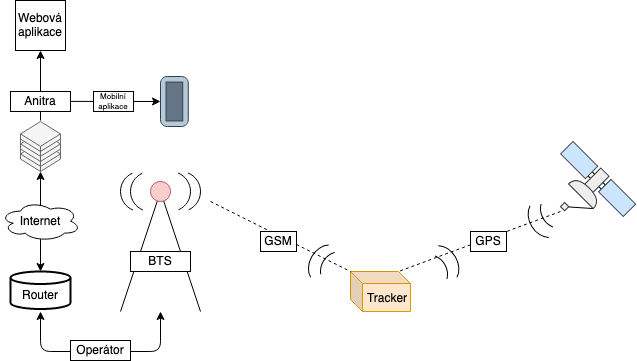
\includegraphics[width=\linewidth]{img/diagram_system.png}
	\caption{Schéma systému GPS-GSM trackerů}
	\label{fig:boat1}
\end{figure}